% flashcards-title: Decimals aligned by place value
% flashcards-desc: A place-value table shows 12.40 above 3.08 with decimal points vertically aligned.
\documentclass[dvisvgm,tikz,border=8pt]{standalone}
\usetikzlibrary{arrows.meta,patterns}

\definecolor{qraNavy}{HTML}{17324D}
\definecolor{qraBlue}{HTML}{2B6CB0}
\definecolor{qraGold}{HTML}{B7791F}
\definecolor{qraPale}{HTML}{EAF2F8}
\definecolor{qraGray}{HTML}{5C6773}

\tikzset{
  qra axis/.style={draw=qraNavy, line width=1.2pt},
  qra tick/.style={draw=qraNavy, line width=1pt},
  qra guide/.style={draw=qraGray, densely dashed, line width=0.8pt},
  qra counter/.style={circle, draw=qraNavy, fill=qraPale, line width=0.9pt, minimum size=7mm, inner sep=0pt},
  qra label/.style={font=\sffamily\bfseries, text=qraNavy},
  qra small label/.style={font=\sffamily, text=qraNavy},
}

\begin{document}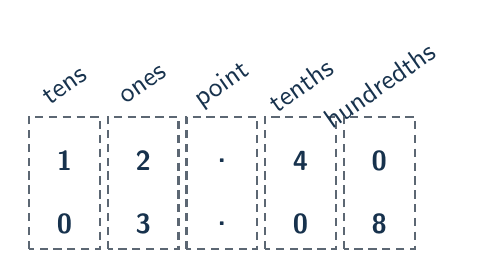
\begin{tikzpicture}[x=1cm,y=.8cm]
\foreach \x/\lab in {0/{tens},1/{ones},2/{point},3/{tenths},4/{hundredths}}{\node[qra small label,rotate=35]at(\x,2.2){\lab};\draw[qra guide](\x-.45,-.4)rectangle(\x+.45,1.7);}
\foreach \x/\v in {0/1,1/2,2/{.},3/4,4/0}{\node[qra label]at(\x,1){\v};}
\foreach \x/\v in {0/0,1/3,2/{.},3/0,4/8}{\node[qra label]at(\x,0){\v};}
\end{tikzpicture}\end{document}
